\GC{I will explore each of the following recommendations in a bit more detail in the final report and will add a summary 
too.}
\section{Summary}
\HD{This is where the overall project summary will go. Aim to keep it pretty brief - 400 to 500 words.}

\section{Future Recommendations}


    \subsection{New Colour Sensors} 
        The colour sensors currently installed on the machine have difficulty in distinguishing between different colours. This is the biggest hindrance to the completion of the project and is the only thing stopping it from being utilised on open days. My recommendation would be to use a camera based system capable of determining the colour of an object in the format of hex-code. Hex-code ranges could be stored within the \acrshort{plc} with each range corresponding to a different colour. With this setup, there is almost a limitless number of colours that could be stored within the \acrshort{plc}, thus, allowing the user to change the secondary hopper colours ad hoc.
    
    \subsection{Extra Functionality} 
        could be added to either the raspberry pi or the Arduino.
    
    \subsection{Replace Cables} 
        that link the auto switch terminals to the remote io so that they are not the same colour as the 24 dc ground.
    
    \subsection{Bump-less Control} 
        between control sources. Currently when you change the control source, i.e., from \acrshort{hmi} to Raspberry-Pi, controller set points may differ.  Ideally, when the control source is altered the controller set-points are maintained. 
    
    \subsection{New Lollies|} 
        Originally, the machine took Allen's Kool Fruits which seemed to work pretty well in regards to size, shape and colour. Unfortunately, Allen's Kool Fruits are now only available in separately packaged plastic bags which for obvious reasons are no good for this application. Currently, the lolly machine is full of gum balls. The gum balls are smaller than Allen's Kool Fruits and do not seem to work quite as well. 
    
    \subsection{Isolation Valve} 
        An isolation valve that feeds all pneumatic control valves, and in turn, depressurises all pneumatic peripherals on the lolly machine. The isolation valve could be part of a safety function linked to the \acrshort{estop}. When the \acrshort{estop} is pressed, all valves are depressurised allowing any trapped objects or body parts to be easily removed from critical pinch/ grab points.

    \subsection{Additional 
        LED Front Panel LED Functions} Can add lights flashing for startup? Could have different levels or Alarms. Could flash orange and green when there is a a Lolly jam. 

    \subsection{Replace Click PLC} \label{sec:replacePlc}
        Use a Siemens \acrshort{plc} instead. As an example of one area where this would improve the control system is the \acrshort{fto} and \acrshort{ftc} logic. Function blocks would drastically improve development time and also would make troubleshooting far better. 

        \begin{figure}[H]
            \centering
            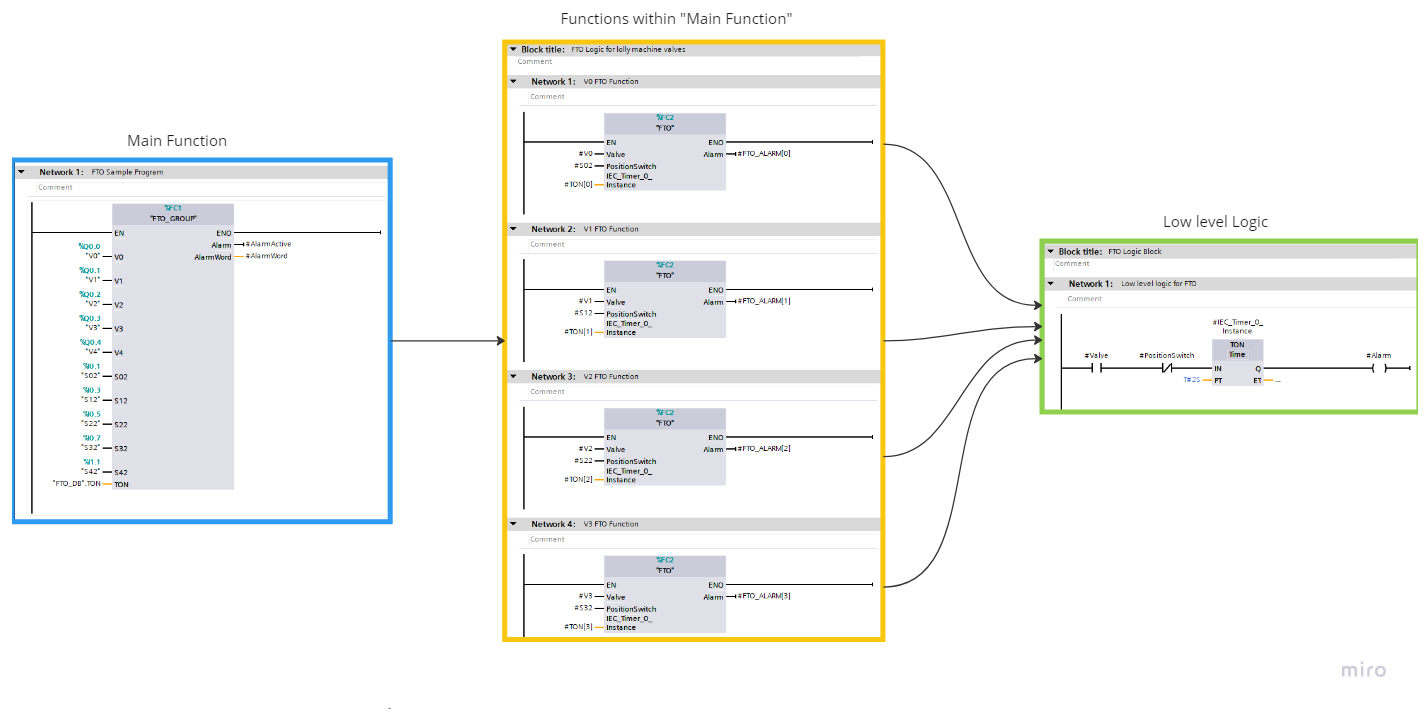
\includegraphics[width = 0.9\textwidth]{2_images/ftoFunTia}
            \caption{An example showing FTO logic using Siemens programming software \acrfull{tia}}
            \label{fig:ftoFunTia}
        \end{figure}



% Given the multifaceted nature of the \textbf{Lolly Machine Upgrade 2} there are many different terms, concepts and ideas that the reader must be aware of prior to understanding the main body of work to follow - the thesis report. This document has aimed to preface the reader with the required knowledge needed to be able to understand the proceeding thesis report. This way, the final body of work can focus on how and what was done rather than stopping ans starting all the time to explain ideas and concepts. Five main topics were discussed in this document. A basic introduction to pneumatics and the relevant devices were reviewed. Various types of \acrshort{io} devices onboard the machine were analysed. Specific components required for automatic machine operation were detailed and discussed and an introduction to relevant communication technologies was made. 